\chapter{Ejemplos de uso de LaTeX}\label{cap:ejemplos}

\todo[inline]{Este capítulo se incluye únicamente como ayuda y referencia de uso de \LaTeX. No debe aparecer en el documento final.}

\section{Introducción}
En este capítulo se muestran ejemplos de uso de \LaTeX{} para operaciones comunes. 

\section{Estilos}\label{sec:estilos}
Se pueden aplicar estilos al texto como \textbf{negritas}, \textit{cursiva}, \underline{subrayado} y \texttt{monoespaciado}. También se \textcolor{red}{pueden} \textcolor{blue}{aplicar} \textcolor{green}{colores}, y \underline{\textit{combinar}} \textbf{\textcolor{red}{estilos}}. Se recomienda usar sólo negritas para hacer énfasis, y no abusar de este recurso.

Por comodidad para usuarios no habituados con LaTeX, esta plantilla define algunos alias de comandos más fáciles de recordar para estilos de texto comunes: \negritas{negritas}, \cursiva{cursiva} y \codigo{código}.

\section{Listados}
Con itemize se pueden crear listas no numeradas:

\begin{itemize}
    \item Fresas
    \item Melocotones
    \item Piñas
    \item Nectarinas
\end{itemize}

De manera similar, enumerate permite crear listas numeradas:

\begin{enumerate}
    \item Elaborar la memoria del TFG
    \item Elaborar la presentación
    \item Presentar el TFG
    \item Solicitar el título de Grado
\end{enumerate}

\section{Subsecciones}
Se pueden definir subsecciones con el comando \texttt{subsection}:

\subsection{Primera subsección}\label{sec:subseccion}
Esto es una subsección

\subsection{Segunda subsección}
Esto es otra subsección.

\subsubsection{Sub-sub-sección}
Este es un tercer nivel de profundidad, que no aparece en el índice general. Se recomienda no utilizarlo, si es posible.

\section{Imágenes y figuras}
Todas las imágenes y figuras del documento se incluirán en la carpeta ``figures''. Se pueden incluir de la siguiente manera:

\begin{figure}[htp]
    \centering
    
\includegraphics[width=0.7\textwidth]{figures/ejemplo.png}
    \caption{Un feroz depredador}
    \label{fig:ejemplo}
\end{figure}

Observe que las figuras se numeran automáticamente según el capítulo y el número de figuras que hayan aparecido anteriormente en dicho capítulo. Existen muchas maneras de definir el tamaño de una figura, pero se aconseja utilizar la mostrada en este ejemplo: se define el ancho de la figura como un porcentaje del ancho total de la página, y la altura se escala automáticamente. De esta manera, el ancho máximo de una figura sería 1.0 * textwidth, lo que aseguraría que se muestra al máximo tamaño posible sin sobrepasar los márgenes del documento.

Tenga en cuenta que LaTeX intenta incluir las figuras en el mismo sitio donde se declaran, pero en ocasiones no es posible por motivos de espacio. En esos casos, LaTeX colocará la figura lo más cerca posible de su declaración, puede que en una página diferente. Esto es un comportamiento normal.

\section{Tablas}
Existe una gran variedad de formas de crear tablas en LaTeX puro, y todas ellas tienen cierta complejidad. A continuación se muestra un ejemplo simple de tabla nativa, en la Tabla \ref{table:ejemplo}. Se recomienda crear un archivo en la carpeta \textit{tables} por cada tabla nativa que se desee incluir, y enlazarla mediante el comando \texttt{input}.

\begin{table}[htp]
\centering

    % Esta primera línea define las columnas de la tabla. Los posibles tipos de columna son:
    % c: texto centrado
    % l: texto alineado a la izquierda
    % r: texto centrado a la derecha
    % p: columna de ancho fijo
    % Las columnas tienen ancho dinámico según la anchura máxima de los elementos que contengan.

    % Las columnas l/r/c no parten el texto en filas diferentes si éste es demasiado largo. Para ello, puede utilizar el tipo de columna de ancho fijo "p".
    
    % Las barras verticales | se usan para definir los bordes verticales de la tabla. Pruebe a eliminar algunas y observe qué ocurre.
    \begin{tabular}{ | l | c | r | p{2cm} | }
        
        % A continuación van las filas de la tabla. En cada fila, las columnas se separan con el carácter &
        % Para terminar una fila se usa \\
        % Para incluir un borde horizontal entre filas se usa \hline

        % Cabecera con textos en negrita:
        \hline
        \textbf{Columna L} & \textbf{Columna C} & \textbf{Columna R} & \textbf{Columna P}\\
        \hline
        
        % Cuerpo de la tabla:
        Texto de ejemplo & Texto de ejemplo & Texto de ejemplo & Texto de ejemplo\\
        \hline
        ABC & DEF & HIJ & KLM\\
        \hline
        
    \end{tabular} 
    
    \caption{Tabla LaTeX de ejemplo}
    \label{table:ejemplo} 
\end{table}


Para tablas con un formato más complejo, considere la posibilidad de diseñarla usando otro software externo (por ejemplo Excel) e incluirla de manera similar a una figura. \textbf{Observe en el código LaTeX a continuación cómo usar el comando \texttt{captionof\{table\}}, en lugar de simplemente \texttt{caption}, hace que se liste como una Tabla en lugar de como una Figura}:

\begin{figure}[htp]
    \centering
    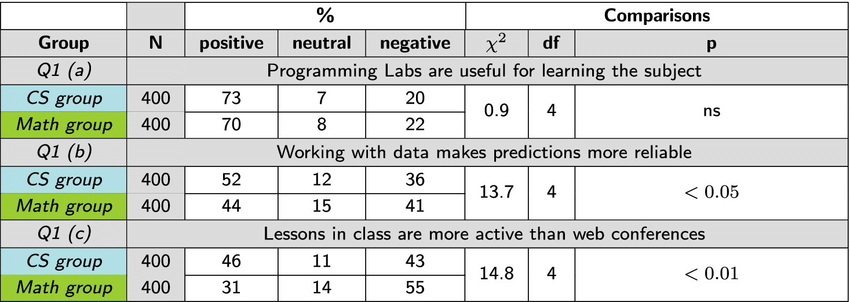
\includegraphics[width=1.0\textwidth]{tables/complex_table.png}
    \captionof{table}{Tabla compleja introducida como figura}
    \label{table:ejemplo2}
\end{figure}

\section{Referencias}
Observe cómo en el código fuente de esta sección se ha usado varias veces el comando \texttt{label}. Este comando permite marcar un elemento, ya sea capítulo, sección, figura, etc. para hacer una referencia numérica al mismo. Para referenciar una label se usa el comando \texttt{ref} incluyendo el nombre de la referencia:

Este es el capítulo \ref{cap:ejemplos}.

En la sección \ref{sec:estilos} se muestran ejemplos de estilos.

La subsección \ref{sec:subseccion} explica...

En la Figura \ref{fig:ejemplo} vemos que...

Esto evita que tengamos que escribir directamente los índices de las secciones y figuras que queremos mencionar, ya que LaTeX lo hace por nosotros y además se encarga de mantenerlos actualizados en caso de que cambien (pruebe a mover este capítulo al final del documento y observe cómo se actualizan automáticamente todos los índices referenciados). Además, las referencias mediante ``ref'' actúan como hipervínculos dentro del documento que llevan al elemento referenciado al pulsar en ellas.

Es habitual nombrar las ``label'' con un prefijo que indica el tipo de elemento para encontrarlo luego más fácilmente, pero no es obligatorio.

\section{Extractos de código}

Se pueden incluir extractos de código mediante lstlisting:

\begin{lstlisting}[language=Python, caption={Código Python}, label={cod:python}, captionpos=b]
num = float(input("Enter a number: "))
if num > 0:
   print("Positive number")
elif num == 0:
   print("Zero")
else:
   print("Negative number")
\end{lstlisting}

Para evitar tener que incluir el código directamente en el texto del documento, se pueden guardar en archivos separados y referenciarlos:

\lstinputlisting[
    float,
    floatplacement=!htp,
    language=Java,
    label=cod:java,
    caption=Código Java
]{code/java_example.java}

\lstinputlisting[
    float,
    floatplacement=!htp,
    language=html,
    label=cod:html,
    caption=Código HTML
]{code/html_example.html}

\lstinputlisting[
    float,
    floatplacement=!htp,
    language=javascript,
    label=cod:js,
    caption=Código JavaScript
]{code/javascript_example.js}

Los extractos de código también se pueden referenciar mediante label/ref: Extractos de código \ref{cod:python}, \ref{cod:java}, \ref{cod:html}, \ref{cod:js}. 

\section{Enlaces}
Puede enlazar una web externa mediante el comando \texttt{url}: \url{https://www.example.com}. También se puede vincular un enlace a un texto mediante el comando href: \href{https://www.example.com}{dominio de ejemplo}.

\section{Citas y bibliografía}
En LaTeX, los elementos de la bibliografía se almacenan en un fichero bibliográfico en un formato llamado BibTeX, en el caso de este proyecto se encuentran en ``bibliografia.bib''. Para citar un elemento se usa el comando \texttt{cite}. Se pueden citar tanto artículos científicos \cite{borrego2019} como enlaces web \cite{webETSII}. 

También se puede usar el comando \texttt{citet} para incluir una referencia junto con el nombre de su autor o autores: \citet{borrego2021}. Todas las citas se numeran automáticamente y se incluyen en la sección de bibliografía del trabajo. El orden por defecto es según su orden de aparición en el documento. Para ordenarlas por orden alfabético del autor, puede modificar el comando \texttt{bibliographystyle} del archivo principal y reemplazar su valor por el estilo \texttt{plainnat} (orden alfabético, nombres completos) o \texttt{abbrvnat} (orden alfabético, nombres abreviados).

Observe cómo los elementos bibliográficos almacenados en ``bibliografia.bib'' tienen una etiqueta asociada, que es la que se usa al citarlos mediante cite. \textbf{Añadir una referencia al fichero bibliográfico no hace que ésta aparezca automáticamente en la sección de bibliografía del trabajo, es necesario citarla en algún lugar del mismo}.

\section{Ecuaciones}
LaTeX tiene un potente motor para mostrar ecuaciones matemáticas y un amplio catálogo de símbolos matemáticos. El entorno matemático se puede activar de muchas maneras. Para incluir ecuaciones simples en un texto se pueden rodear de símbolos dólar: $1 + 2 = 3$, $\sqrt{81} = 3^2 = 9$, $\forall x \in y~\exists~z : S_z < 4$.

Las ecuaciones más complejas pueden expresarse aparte y son numeradas: ecuación \ref{eq:ecuacion}.

\begin{equation}\label{eq:ecuacion}
\lim_{x\to 0}{\frac{e^x-1}{2x}}
 \overset{\left[\frac{0}{0}\right]}{\underset{\mathrm{H}}{=}}
 \lim_{x\to 0}{\frac{e^x}{2}}={\frac{1}{2}}
 +7 \int_0^2
  \left(
    -\frac{1}{4}\left(e^{-4t_1}+e^{4t_1-8}\right)
  \right)\,dt_1
\end{equation}

Dispone \href{http://www.yann-ollivier.org/latex/texsymbols.pdf}{aquí} de un amplio listado de símbolos que pueden usarse en modo matemático.

\section{Caracteres y símbolos especiales}
Algunos caracteres y símbolos deben ser escapados para poder representarse en el documento, ya que tienen un significado especial en LaTeX. Algunos de ellos son:

\begin{itemize}
    \item El símbolo dólar \$ se usa para ecuaciones.
    \item El tanto por ciento \% se usa para comentarios en el código fuente.
    \item El símbolo euro \euro{} suele dar problemas si se escribe directamente.
    \item El guión bajo \_ se usa para subíndices en modo matemático.
    \item Las comillas deben expresarse `así' para comillas simples y ``así'' para comillas dobles. Las comillas españolas pueden expresarse \textquote{así}.
    \item La barra invertida o contrabarra \textbackslash{} se usa para comandos LaTeX.
    \item Otros símbolos que deben escaparse son las llaves \{ \}, el ampersand \&, la almohadilla \# y los símbolos mayor que \textgreater{} y menor que \textless{}.
\end{itemize}